\documentclass{beamer}
\usepackage{mathtools}
\usepackage{amsmath}
\usepackage{listings}
\usetheme{CambridgeUS}

\title{Optimization}
\author{Sandeep H M \and Dinesh Kumar Sonkar}
\date{\today}
\subject{EE5327 - Optimization}

\AtBeginSubsection[]
{
  \begin{frame}<beamer>{Outline}
    \tableofcontents[currentsection,currentsubsection]
  \end{frame}
}

% Let's get started
\begin{document}

\begin{frame}
  \titlepage
\end{frame}

\section{Problem}
\begin{frame}{Problem}
\begin{block}{Problem Statement}
Maximize
\begin{equation*}
    f(\textbf{X}) = \sqrt{x_{1}*x_{2}}
\end{equation*}
subject to the constraints\\
\begin{equation*}
x_{1}^{2} + x_{2}^{2} \leq 5
\end{equation*}
\begin{equation*}
x_{1}\geq 0,x_{2}\geq 0
\end{equation*}
\end{block}

\begin{figure}
\centering
    \subfloat{{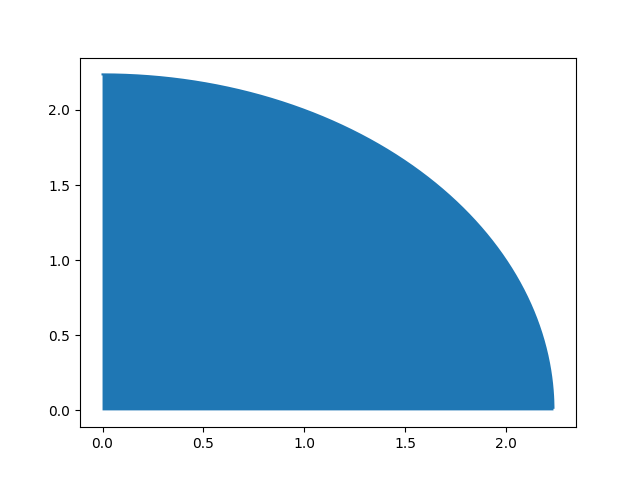
\includegraphics[width=3cm]{Area.png}}}
    \qquad
    \subfloat{{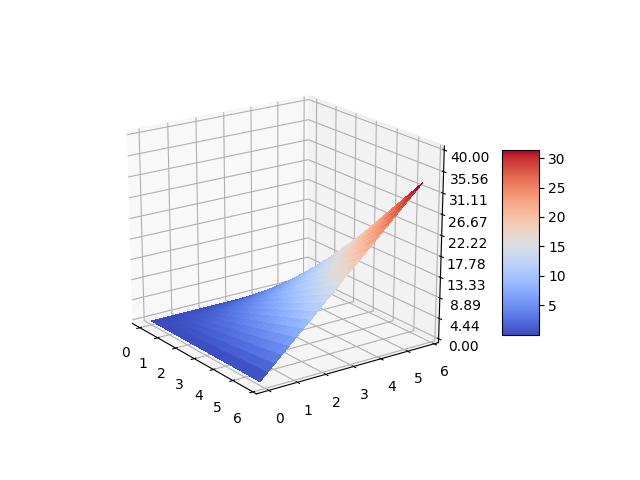
\includegraphics[width=3cm]{x1x2.png}}}
    \label{fig:example}
\end{figure}
\end{frame}

\section{Lagrange Multiplier} 
\begin{frame}{Lagrange Multiplier}
Consider the problem optimization problem
\begin{equation*}
    \min_{x} f(\textbf{x}), g(\textbf{x})\leq 0
\end{equation*}
The Lagrangian is 
\begin{equation*}
   \mathcal{L}(\textbf{x},\lambda) = f(\textbf{x}) + \lambda g(\textbf{x})
\end{equation*}
We find $\nabla \mathcal{L}(\textbf{x},\lambda)$ and set it to 0.\\
If $\lambda$ obtained after solving is positive, the solution is correct.\\
Else set $\lambda$ = 0
\end{frame}

\section{Solution}
\begin{frame}{Solution}
Considering the Lagrangian\\
\begin{equation*}
\mathcal{L}(\textbf{X},\lambda)= -\sqrt{x_{1}x_{2}} + \lambda( x_{1}^{2} + x_{2}^{2} - 5)
\end{equation*}
\\
\begin{equation*}
\nabla\mathcal{L}(\textbf{X},\lambda)=
    \begin{bmatrix}
    \displaystyle\frac{-\sqrt{x_{2}}}{2\sqrt{x_{1}}} + 2\lambda x_{1}\\
    \\
    \displaystyle\frac{-\sqrt{x_{1}}}{2\sqrt{x_{2}}} + 2\lambda x_{2}\\
    \\
    x_{1}^{2} + x_{2}^{2} - 5
\end{bmatrix}
\end{equation*}
\\
To find optimal values of $x_{1}$ and $x_{2}$ we set 
\begin{equation*}
\nabla\mathcal{L}(\textbf{X},\lambda)=0
\end{equation*}
\end{frame}

\begin{frame}

\begin{equation}
\displaystyle\frac{\sqrt{x_{2}}}{2\sqrt{x_{1}}} = 2\lambda x_{1}
\end{equation}
\begin{equation*}
\implies \lambda=\displaystyle\frac{\sqrt{x_{2}}}{4x_{1}^{\frac{3}{2}}}     
\end{equation*}

\begin{equation}
     \displaystyle\frac{-\sqrt{x_{1}}}{2\sqrt{x_{2}}} + 2\lambda x_{2}
\end{equation}
\begin{equation*}
\implies \lambda=\displaystyle\frac{\sqrt{x_{1}}}{4x_{2}^{\frac{3}{2}}}
\end{equation*}

\begin{equation*}
   \frac{\sqrt{x_{2}}}{4x_{1}^{\frac{3}{2}}}=  \frac{\sqrt{x_{1}}}{4x_{2}^{\frac{3}{2}}}  
\end{equation*}
\begin{equation*}
x_{1}^{2} = x_{2}^{2}
\implies x_{1} = x_{2}
\end{equation*}
\end{frame}

\begin{frame}
Substituting $x_{1} = x_{2}$ in the equation
\begin{equation}
 x_{1}^{2} + x_{2}^{2} = 5
\end{equation}
We get
\begin{equation*}
    2x_{1}^{2} = 5
\end{equation*}
\begin{equation*}
\implies x_{1}=x_{2}=\displaystyle\sqrt{\frac{5}{2}}
\end{equation*}

Maximum value of f(\textbf{X}) is
\begin{equation*}
   \displaystyle f_{max}(\textbf{X})=\sqrt{\sqrt{\frac{5}{2}}*\sqrt{\frac{5}{2}}} = \sqrt{\frac{5}{2}} = 1.5811 
\end{equation*}
Maximum value is 1.5811
\end{frame}

\section{Solution using CVXPY}

\begin{frame}{Solution using CVXPY}
\lstinputlisting[language=Python]{Presentation_3.16.py}

Maximum value = 1.581138\\
$x_{1} = x_{2} = 1.581138$
\end{frame}

\end{document}


